\documentclass[a4paper,twoside]{article}
\usepackage[T1]{fontenc}
\usepackage[bahasa]{babel}
\usepackage{graphicx}
\usepackage{graphics}
\usepackage{float}
\usepackage[cm]{fullpage}
\pagestyle{myheadings}
\usepackage{etoolbox}
\usepackage{setspace} 
\usepackage{lipsum} 
\setlength{\headsep}{30pt}
\usepackage[inner=2cm,outer=2.5cm,top=2.5cm,bottom=2cm]{geometry} %margin
% \pagestyle{empty}

\makeatletter
\renewcommand{\@maketitle} {\begin{center} {\LARGE \textbf{ \textsc{\@title}} \par} \bigskip {\large \textbf{\textsc{\@author}} }\end{center} }
\renewcommand{\thispagestyle}[1]{}
\markright{\textbf{\textsc{Laporan Perkembangan Pengerjaan Skripsi\textemdash Sem. Genap 2021/2022}}}

\onehalfspacing
 
\begin{document}

\title{\@judultopik}
\author{\nama \textendash \@npm} 

%ISILAH DATA BERIKUT INI:
\newcommand{\nama}{Edwin Pranajaya}
\newcommand{\@npm}{2017730027}
\newcommand{\tanggal}{21/06/2021} %Tanggal pembuatan dokumen
\newcommand{\@judultopik}{Dukungan Bahasa JavaScript pada SharIF Judge} % Judul/topik anda
\newcommand{\kodetopik}{PAN5291}
\newcommand{\jumpemb}{1} % Jumlah pembimbing, 1 atau 2
\newcommand{\pembA}{Pascal Alfadian Nugroho}
\newcommand{\pembB}{-}
\newcommand{\semesterPertama}{52 - Genap 21/22} % semester pertama kali topik diambil, angka 1 dimulai dari sem Ganjil 96/97
\newcommand{\lamaSkripsi}{1} % Jumlah semester untuk mengerjakan skripsi s.d. dokumen ini dibuat
\newcommand{\kulPertama}{Skripsi 1} % Kuliah dimana topik ini diambil pertama kali
\newcommand{\tipePR}{B} % tipe progress report :
% A : dokumen pendukung untuk pengambilan ke-2 di Skripsi 1
% B : dokumen untuk reviewer pada presentasi dan review Skripsi 1
% C : dokumen pendukung untuk pengambilan ke-2 di Skripsi 2

% Dokumen hasil template ini harus dicetak bolak-balik !!!!

\maketitle


\pagenumbering{arabic}

\section{Data Skripsi} %TIDAK PERLU MENGUBAH BAGIAN INI !!!
Pembimbing utama/tunggal: {\bf \pembA}\\
Pembimbing pendamping: {\bf \pembB}\\
Kode Topik : {\bf \kodetopik}\\
Topik ini sudah dikerjakan selama : {\bf \lamaSkripsi} semester\\
Pengambilan pertama kali topik ini pada : Semester {\bf \semesterPertama} \\
Pengambilan pertama kali topik ini di kuliah : {\bf \kulPertama} \\
Tipe Laporan : {\bf \tipePR} -
\ifdefstring{\tipePR}{A}{
			Dokumen pendukung untuk {\BF pengambilan ke-2 di Skripsi 1} }
		{
		\ifdefstring{\tipePR}{B} {
				Dokumen untuk reviewer pada presentasi dan {\bf review Skripsi 1}}
			{	Dokumen pendukung untuk {\bf pengambilan ke-2 di Skripsi 2}}
		}
		
\section{Latar Belakang}
SharIF-Judge adalah \textit{online judge} gratis dan open source untuk bahasa pemrograman C, C++, Java dan Python. SharIF-Judge merupakan hasil \textit{fork} dari SharIF-Judge asli yang dibuat oleh Mohammad Javad Naderi. Versi bercabang ini mengandung banyak perbaikan, sebagian besar karena kebutuhan fakultas Informatika UNPAR.

SharIF-Judge biasa digunakan untuk mempermudah evaluasi kode program.  SharIF-Judge digunakan pada beberapa kuliah di Informatika(IF), seperti Dasar Pemrograman dan Algoritma Struktur Data. Tujuan SharIF-Judge digunakan pada perkuliahan, adalah agar dapat mempermudah kegiatan belajar mengajar berlangsung. Mahasiswa dapat dengan mudah melakukan pengiriman kode program atau \textit{file} ke SharIF-Judge dan dapat langsung melihat nilainya. Pengajar yang bertanggung jawab atas kegiatan belajar mengajar tersebut tidak akan kesusahan dalam mengumpulkan hasil pekerjaan para pelajar. 

Alur dari penggunaan SharIF-Judge ini diawali dengan pengajar yang membuat soal terlebih dahulu. Setelah soal disiapkan, pengajar dapat membuat \textit{assignment} dengan click tombol \textit{add assignment}. Didalamnya, pengajar diwajibkan untuk memasukan nama \textit{assignment}, waktu dimulainya pengerjaan, waktu selesai pengerjaan, waktu tambahan pengerjaan, daftar peserta, deskripsi soal, dan kunci jawaban dari soal yang sudah dibuat oleh pengajar. Meskipun SharIF-Judge dapat membaca berbagai bahasa pemrograman, JavaScript bukan salah satu yang dapat dibaca oleh SharIF-Judge.

JavaScript adalah bahasa skrip sisi klien yang berjalan sepenuhnya di dalam \textit{browser web}. Sebagai contoh dapat dilihat \textit{menu drop-down} yang mencolok, memindahkan teks, dan mengubah konten yang sekarang tersebar luas di situs web. Semua interaksi tersebut diaktifkan melalui JavaScript. Berdasarkan survey yang diberikan pada stackoverflow pada tahun 2021, selama 9 tahun berturut-turut, JavaScript merupakan bahasa pemrograman yang paling sering digunakan. 64,96\% developer dari 83,052 responden di dunia menggunakannya.

Berdasarkan data diatas, ditunjukan bahwa JavaScript termasuk dalam bahasa pemrograman yang sangat populer dan banyak digunakan. Sangat disayangkan jika SharIF Judge tidak dapat membaca bahasa tersebut. Akan kesulitan bagi para pengajar karena harus mengikuti perkembangan zaman, namun pemeriksaannya tidak mudah. Kostumisasi dari SharIF Judge akan dilakukan agar \textit{online judge} tersebut dapat membaca JavaScript. Untuk mempermudah kostumasi, pengerjaan akan dilakukan dengan menggunakan OS Linux. Namun dikarenakan OS yang digunakan adalah Windows, akan digunakan \textit{virtual machine} agar dapat mengerjakan dengan OS Linux pada Windows. 

\section{Rumusan Masalah}
Berdasarkan latar belakang tersebut, maka rumusan masalah penelitian sebagai berikut: 

     Bagaimanakah cara agar SharIF-Judge dapat memahami bahasa pemrograman JavaScript untuk dievaluasi.

\section{Tujuan}
Berdasarkan rumusan masalah, maka tujuan penelitian ini adalah sebagai berikut:

    Melakukan modifikasi pada SharIF-Judge agar dapat menerima soal JavaScript dan dapat melakukan evaluasi pada JavaScript.


\section{Detail Perkembangan Pengerjaan Skripsi}
Detail bagian pekerjaan skripsi sesuai dengan rencan kerja/laporan perkembangan terkahir :
	\begin{enumerate}
        \item \textbf{Melakukan instalasi pada SharIF-Judge}\\
		{\bf Status :} Ada sejak rencana kerja skripsi.\\
		{\bf Hasil :} Instalasi SharIF-Judge dilakukan melalui github yang dimiliki oleh Informatika UNPAR. Untuk dapat menjalankan SharIF-Judge, diwajibkan untuk memiliki server Linux dan mengikuti persyaratan sebagai berikut:
\begin{itemize}
    \item Menjalankan PHP versi 5.3 atau versi yang lebih baru.
    \item Pengguna dapat menjalankan PHP dari command line  dan pengguna perlu menginstall paket PHP CLI.
    \item Memiliki \textit{Mysql} atau \textit{PostgreSql database}.
    \item PHP memiliki akses untuk menjalankan perintah \textit{shell} terutama untuk fungsi \textit{shell\_exec}.
    \item Untuk melakukan proses kompilasi dan menjalankan kode yang dikumpulkan adalah (\textit{gcc, g++, javac, java, python2, python3 commands})
    \item Disarankan untuk melakukan instalasi \textit{Perl} dengan alasan agar memiliki ketepatan waktu, penggunaan \textit{memory} yang terbatas dan memaksimalkan batas ukuran pada \textit{output} kode yang dikirimkan.
\end{itemize}
Jika persyaratan diatas telah selesai dilakukan, dapat dilanjutkan untuk melakukan instalasi sebagai berikut: 
\begin{itemize}
    \item Mengunduh versi terakhir dari Sharif Judge dan unpack file yang berhasil diunduh, letakan pada direktori html publik
    \item Untuk mempermudah pindahkan folder \textit{system}  dan \textit{application} keluar dari direktori publik dan masukan \textit{path} lengkap pada file index.php

\begin{verbatim}
        $system_path = `/home/mohammad/secret/system`;
        $application_folder = `/home/mohammad/secret/application`;
\end{verbatim} 
    \item Membuat sebuah \textit{Mysql} atau \textit{PostgreSql database} untuk Sharif Judge.
    \item Mengatur koneksi database di file application/config/database.php.

\begin{verbatim}
/* Enter database connection settings here: */
`dbdriver' => `postgre', // database driver (mysqli, postgre)
`hostname' => `localhost', // database host
`username' => `, // database username
`password' => `, // database password
`database' => `, // database name
`dbprefix' => `shj_', // table prefix
/**********************************************/
\end{verbatim} 


    \item Membuat direktori application/cache/Twig agar dapat ditulis oleh PHP
    \item Membuka halaman utama SharIF-Judge pada web browser \item \textit{Log in}  menggunakan akun \textit{admin}
    \item Memindahkan folder \textit{tester} dan \textit{assigments} di luar direktori publik lalu simpan \textit{path} lengkap pada halaman \textit{Settings} . Dua folder tersebut harus dapat ditulis oleh PHP. File-file yang diunggah akan disimpan di folder \textit{assigments} sehingga tidak dapat diakses publik.
\end{itemize}
	\item \textbf{Menulis dokumen skripsi}\\
		{\bf Status :} Ada sejak rencana kerja skripsi.\\
		{\bf Hasil :} Dokumen skripsi telah dituliskan hingga Bab 3 yaitu analisis sistem kini dan analisis sistem usulan.

		\item \textbf{Mempelajari javascript}\\
		{\bf Status :} Ada sejak rencana kerja skripsi.\\
		{\bf Hasil :} Melakukan studi mengenai javascript. Javascript berfungsi untuk membantu membuat fungsionalitas pada halaman web, sedangkan HTML dan CSS membantu membuat desain halaman web. Javascript memiliki beberapa fungsi yang dapat digunakan, yaitu
		\begin{itemize}
		    \item \textbf{\textit{String}}. Merupakan nilai yang terdiri dari teks dan dapat berisi huruf, angka, simbol, tanda baca, dan emoji. berikut merupakan contoh kode	
		    \begin{verbatim}
EXAMPLE		  
’This is a string.’
		    \end{verbatim}
		    \vspace{-5mm}
		    \item \textbf{\textit{Numbers}}. Merupakan nilai yang dapat digunakan dalam operasi matematika
		    \begin{verbatim}
EXAMPLE		    
12345;
		    \end{verbatim}
		    \vspace{-5mm}
		    \item \textbf{\textit{Booleans}}. Merupakan nilai yang dapat berupa TRUE atau FALSE dimana nilai ini berarti hanya antara benar atau salah
		    \begin{verbatim}
EXAMPLE
var kitchenLights = false;
kitchenLights = true;
kitchenLights;
OUTPUT:
true
		    \end{verbatim}
		    \vspace{-5mm}
		    \item \textbf{\textit{Operators}}. Simbol antara nilai yang memungkinkan operasi yang berbeda seperti penambahan,pengurangan, perkalian, dll.
		    \begin{verbatim}
EXAMPLE:
1+2;
OUTPUT:
3
		    \end{verbatim}
		    \vspace{-5mm}

		    \item \textbf{\textit{Variables}}. Merupakan sesuatu yang akan dideklarasikan.
		    \begin{verbatim}
EXAMPLE
var x = 100;		        
		    \end{verbatim}
		    \vspace{-5mm}
		    \item \textbf{\textit{Functions}}. Merupakan  blok kode yang dapat digunakan kembali yang melakukan tugas tertentu, mengambil beberapa bentuk input dan mengembalikan output.
		    \begin{verbatim}
EXAMPLE
function addTwoNumbers(x, y) {
    return x + y;
}		        
		    \end{verbatim}
		    \vspace{-5mm}
		    \item \textbf{\textit{Conditionals}}. Merupakan cara untuk engontrol perilaku dalam JavaScript dan menentukan apakah potongan kode dapat dijalankan atau tidak.
		    \begin{verbatim}
    EXAMPLE:
    if (10 > 5) {
    var outcome = "if block";
    }
    outcome;
    OUTPUT:
    "if block"		        
		    \end{verbatim}
		    \vspace{-2mm}		    
		    \item \textbf{\textit{Arrays}}. Merupakan nilai seperti wadah yang dapat menampung nilai, Elemen pada array tidak semuanya harus memiliki tipe nilai yang sama. Elemen dapat berupa nilai JavaScript apa pun bahkan array lain.
		    \begin{verbatim}
EXAMPLE:
    var breakfast = ["coffee", "croissant"];
    breakfast;
    OUTPUT:
    ["coffee", "croissant"]			        
		    \end{verbatim}
		    \vspace{-2mm}
	    
		    \item \textbf{\textit{Objects}}. Merupakan variabel yang berisi beberapa nilai data. ata. Nilai dalam objek JavaScript dikenal sebagai properti. 
		    \begin{verbatim}
EXAMPLE:
    var hodgepodge = [100, "paint", [200, "brush"], false];
    hodgepodge;
    OUTPUT:
    [100, "paint", [200, "brush"], false]		        
		    \end{verbatim}
		    \vspace{-2mm}
		    
		    \item \textbf{\textit{Input and Output}}. Untuk javascript, diperlukan menggunakan Modul \textit{Readline}. pada Node.js Modul \textit{Readline} memungkinkan pembacaan aliran input baris demi baris.
		    \begin{verbatim}
var readline = require('readline');
		    \end{verbatim}
		    \vspace{-2mm}
		    
		    \end{itemize}

		\item \textbf{Melakukan kostumisasi pada SharIF-Judge}\\
		{\bf Status :} ada sejak rencana kerja skripsi \\
		{\bf Hasil :} Sudah memberikan perubahan pada tampilan sehingga pengguna dapat memilih \textit{javascript} namun belum memiliki fungsi. Hal tersebut dikarenakan ditemukan bug  sehingga diprioritaskan dokumen dan dilanjutkan pada skripsi 2. Bug yang ditemukan seperti: 
		    \begin{itemize}
		        \item Ketika ingin memasukan file \textit{test case} muncul error yang disebabkan pada config.php terdapat typo
		        \item Ketika \textit{add assignment} dan memasukan \textit{test case}, \textit{test case tersebut} dikatakan file not found. Hal ini disebabkan oleh \textit{End of Line Sequence} pada \textit{tester.sh} yang berawalan dari tipe CLRF dan dirubah menjadi LF. CR LF adalah singkatan dari "Carriage Return, Line Feed" yang merupakan sisa digital dari mesin tik klasik. Dengan mesin tik, Pengguna harus mendorong "carriage" (benda yang menahan kertas) kembali ke tempatnya, maka "Carriage Return". Sedangkan LF memindahkan kursor ke bawah ke baris berikutnya tanpa kembali ke awal baris.
		    \end{itemize}
	
	    \item \textbf{Melakukan eksplorasi pada  SharIF-Judge}\\
		{\bf Status :} Ada sejak rencana kerja skripsi.\\
-		{\bf Hasil :} SharIF-Judge adalah \textit{online judge} gratis dan open source untuk bahasa pemrograman C, C++, Java dan Python. SharIF-Judge merupakan hasil \textit{fork} dari Sharif Judge yang dibuat oleh Mohammad Javad Naderi. Versi bercabang ini mengandung banyak perbaikan, sebagian besar karena kebutuhan fakultas Informatika UNPAR. Antarmuka web ditulis dalam PHP (kerangka CodeIgniter) dan backend utama ditulis dalam BASH.-Python di SharIF Judge belum di-sandbox. Hanya tingkat keamanan rendah yang disediakan untuk python. SharIF-Judge dibuat dengan menggunakan sebuah \textit{framework} yang bernama CodeIgniter. CodeIgniter merupakan framework PHP dengan memiliki arsitektur MVC(Model, View, Controller) untuk mempermudah pembangunan web. Berikut ini merupakan fitur-fitur dari SharIF-Judge:
\begin{figure}[h!]
     \centering
     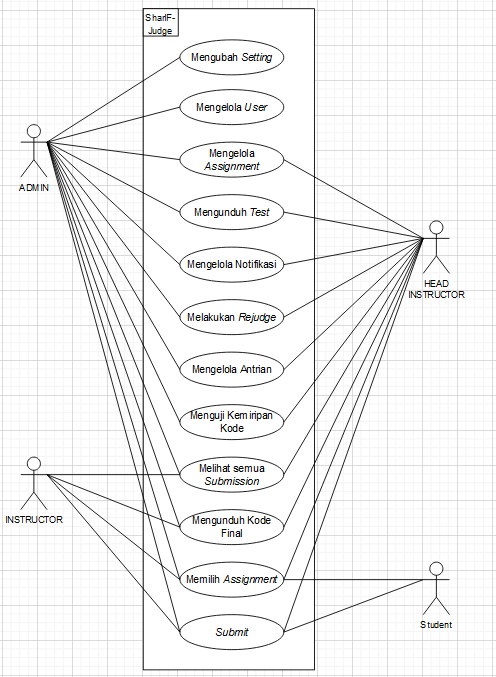
\includegraphics[width=0.5\linewidth]{Gambar/Usecase Diagram.PNG}
     \caption{\textit{Use Case Diagram}}
     \label{fig:Use Case Diagram}
 \end{figure}\newline
Pada Gambar \ref{fig:Use Case Diagram} ditunjukan bahwa terdapat 4 \textit{role} pada SharIF-Judge dari yang memiliki fungsi paling banyak hingga paling sedikit berturut-turut yaitu Admin, \textit{Head Instructor}, \textit{Instructor}, dan \textit{Student}.

\newpage
\begin{figure}[h!]
     \centering
     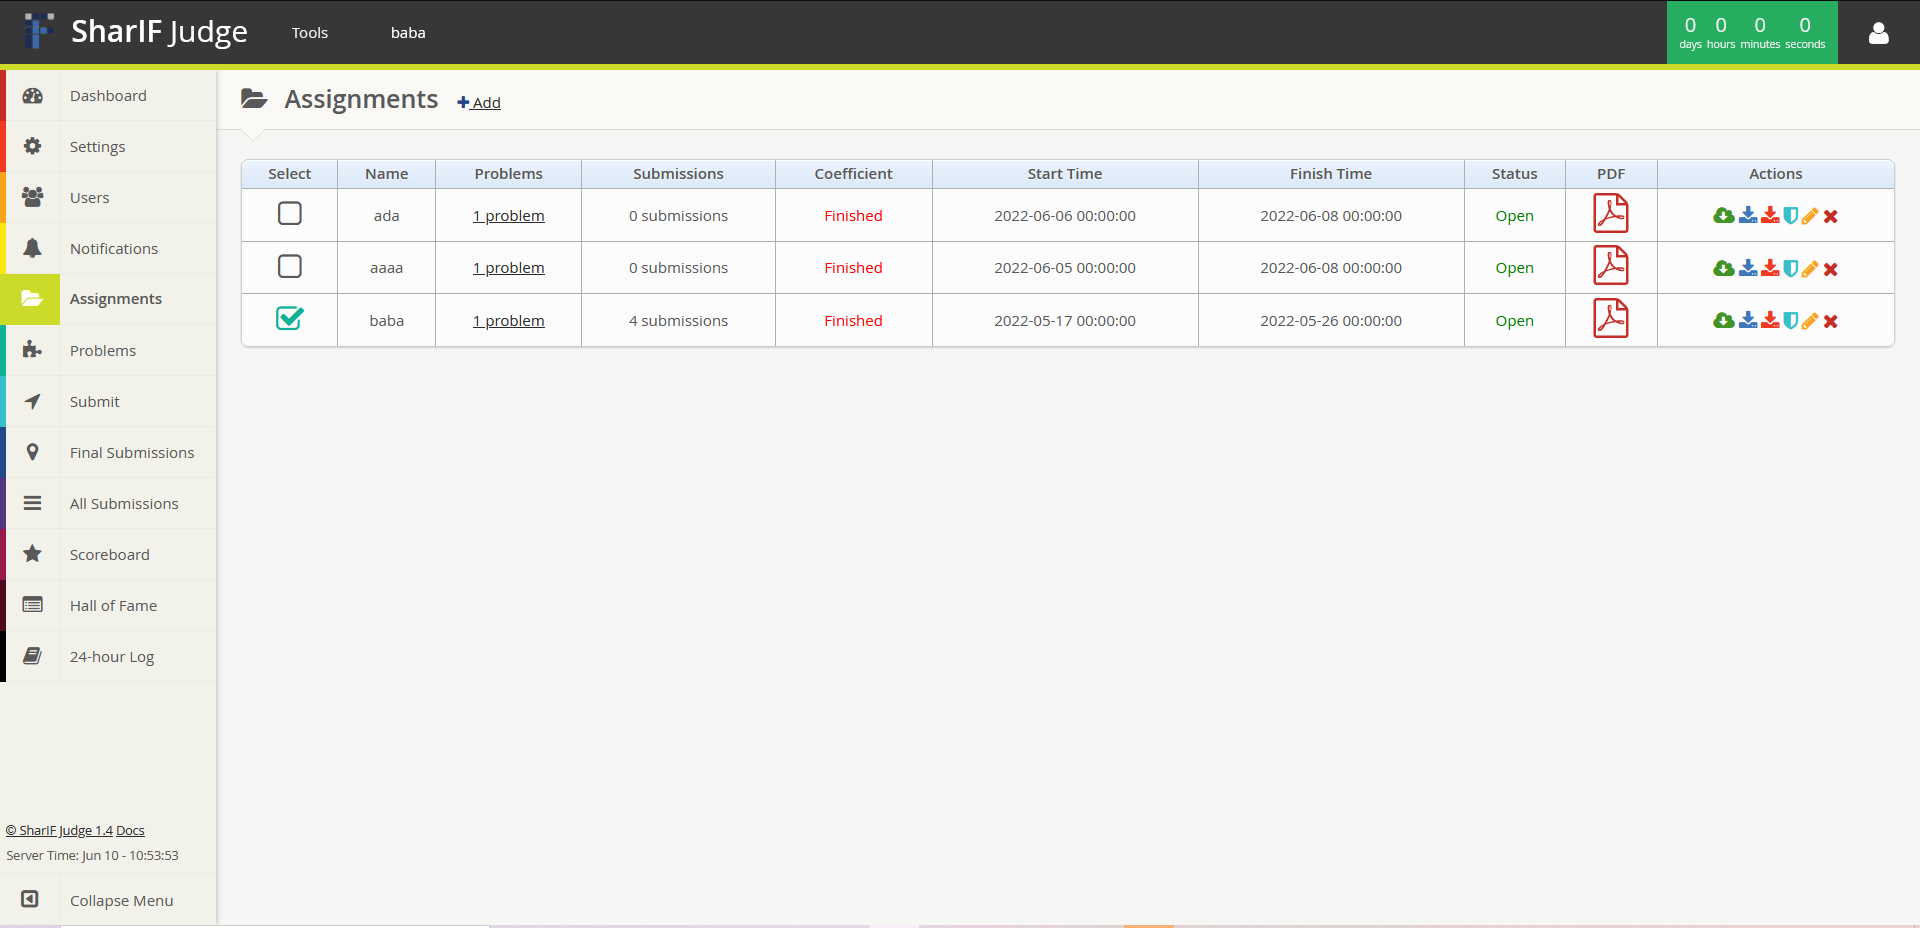
\includegraphics[width=0.8\linewidth]{Gambar/Assignment.png}
     \caption{Halaman \textit{Assignment}}
     \label{fig:Assignment}
 \end{figure}	
 Pada Gambar \ref{fig:Assignment} merupakan halaman \textit{Assignment}, bagi role \textit{student}  halaman \textit{assignment} ini berfungsi sebagai tempat untuk melihat seluruh \textit{assignment} yang ada dan dapat memilih salah satunya. Namun, untuk \textit{role} Admin, dan \textit{Head Instructor} halaman \textit{assignment} dapat berguna untuk menambahkan \textit{assignment} pada \textit{add assignment}, edit, atau bahkan menghapus \textit{assignment}. 
 
 \begin{figure}[h!]
     \centering
     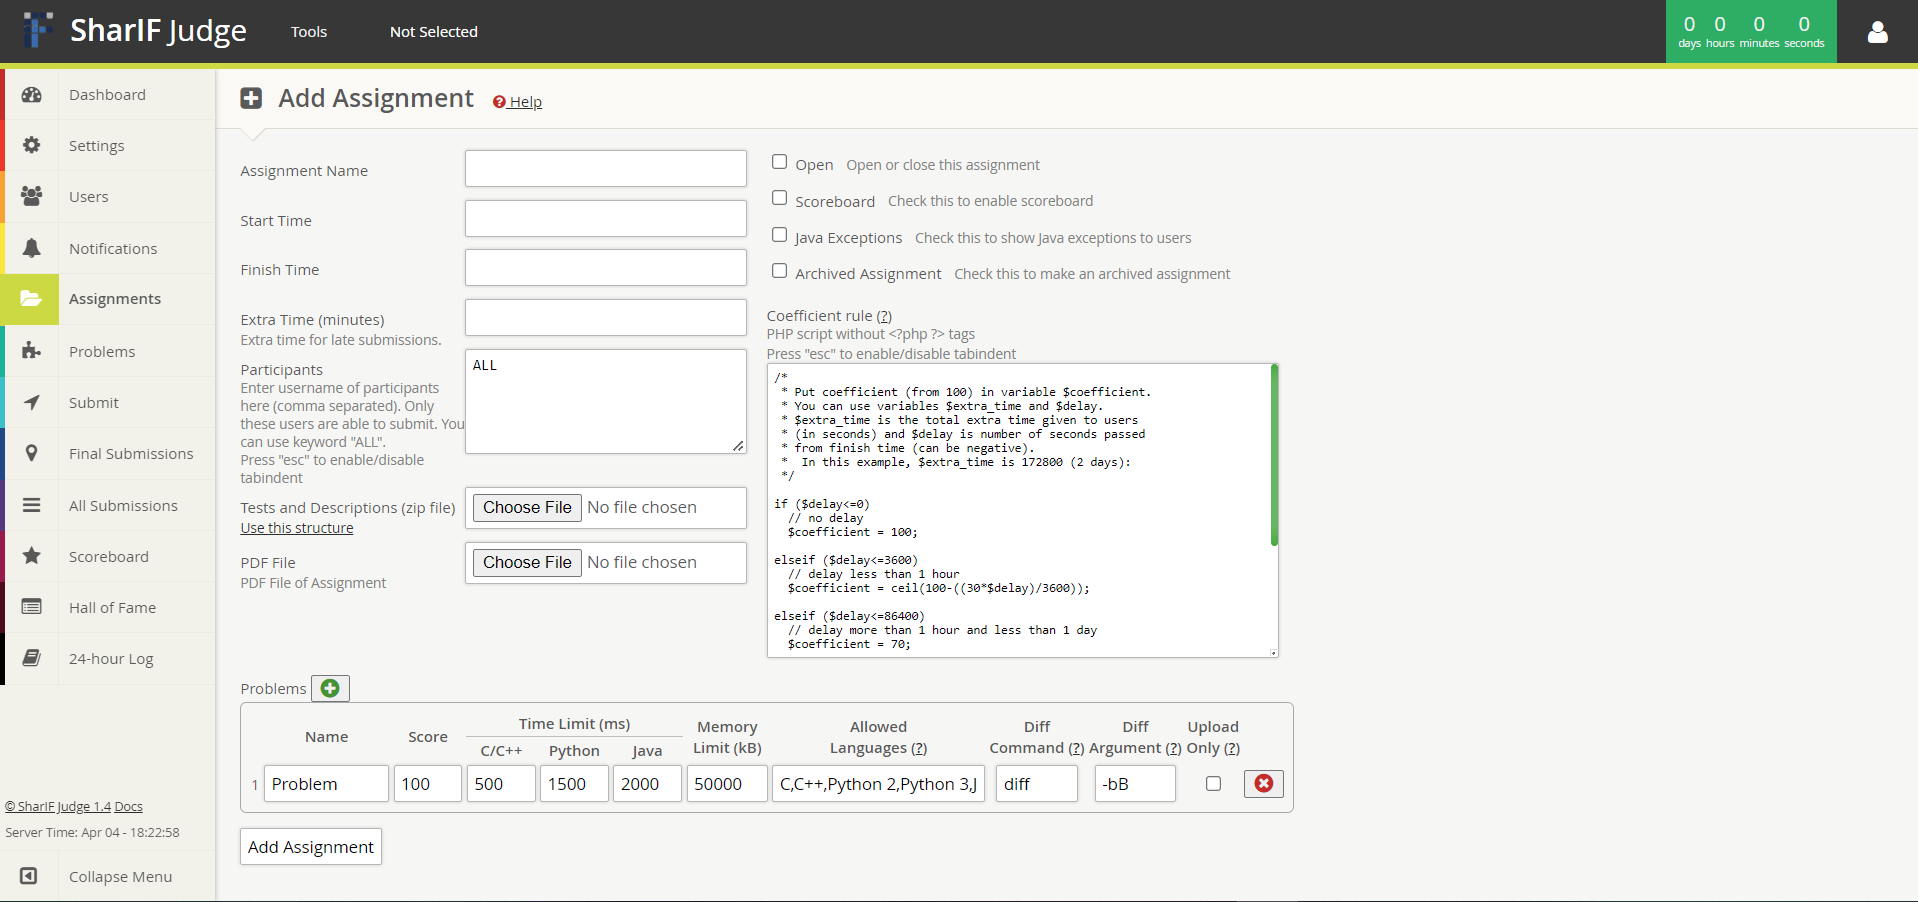
\includegraphics[width=0.8\linewidth]{Gambar/Add Assignment.PNG}
     \caption{Halaman \textit{Add Assignment}}
     \label{fig:addAss}
 \end{figure}
 Gambar \ref{fig:addAss} merupakan halaman pada \textit{Add Assignment}. Halaman tersebut memiliki fungsi untuk Admin dan \textit{Head Instructor} menambahkan \textit{Assignment}. Pada bagian \textit{Allowed Language}, akan dilakukan kostumisasi agar javascript menjadi salah satu bahasa yang diterima oleh SharIF-Judge.
 \newpage
  \begin{figure}[h!]
     \centering
     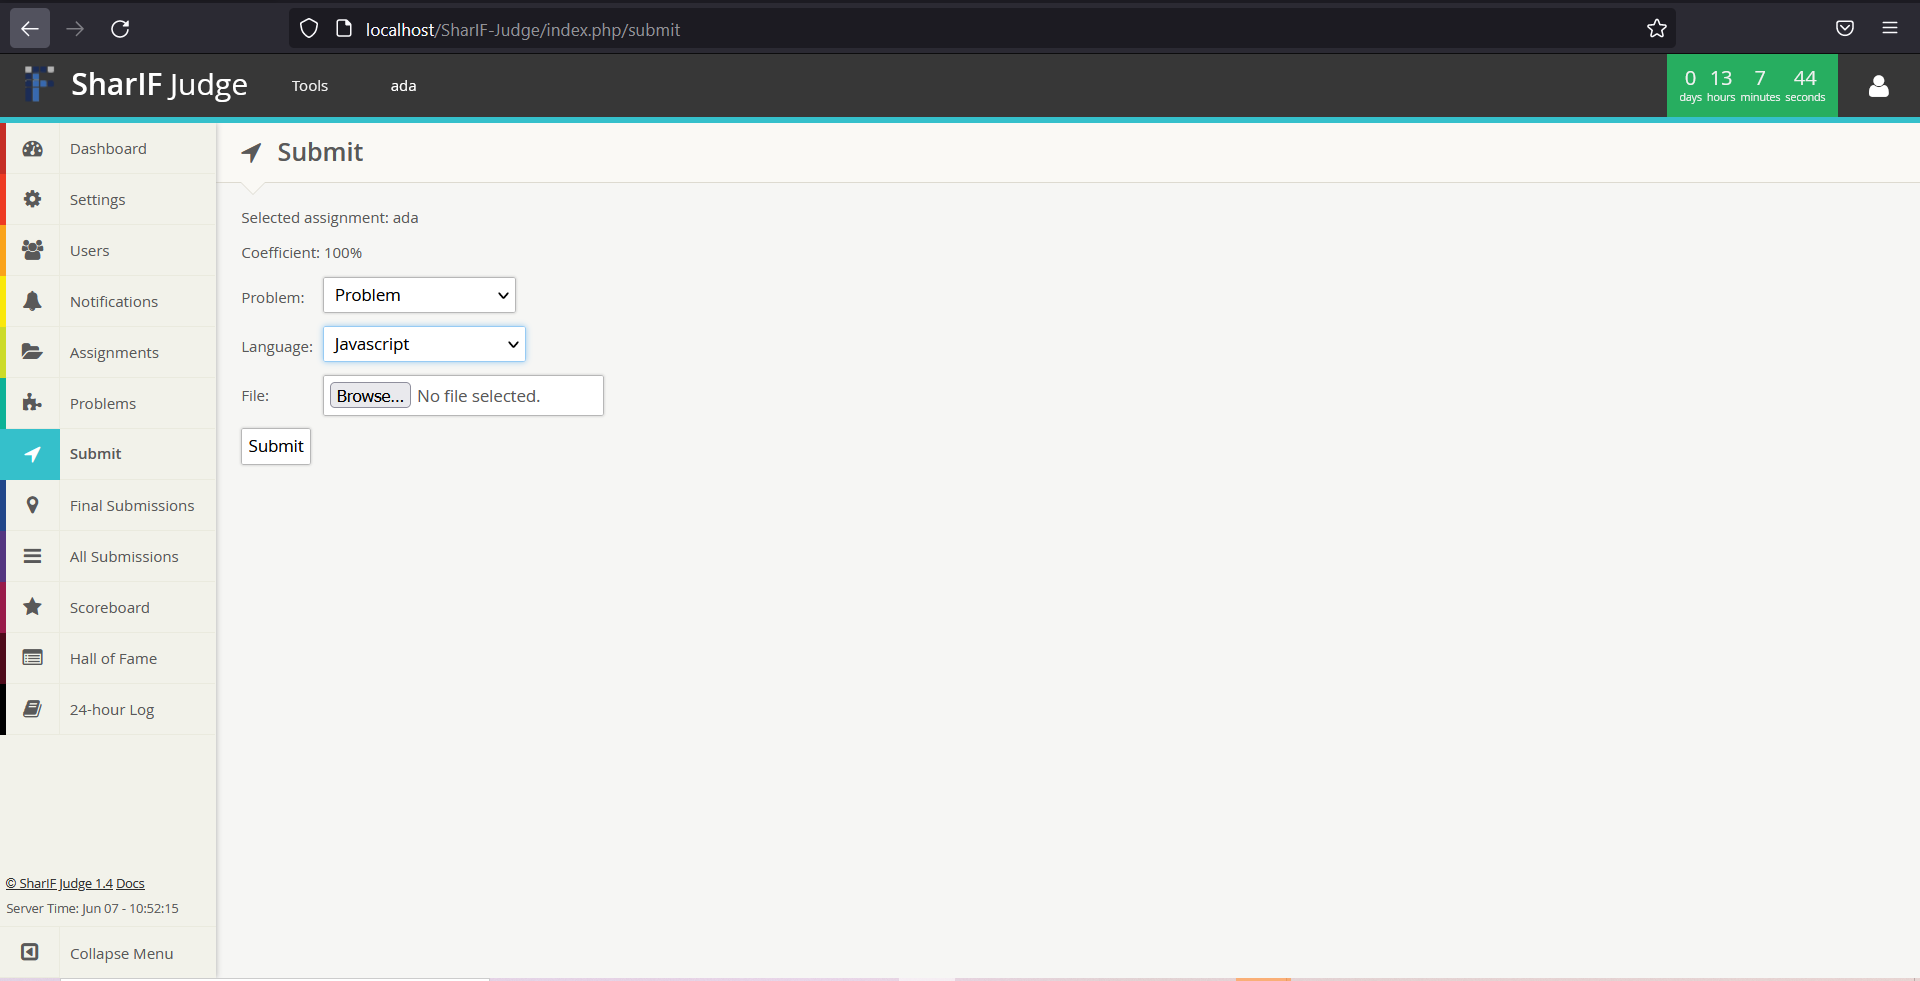
\includegraphics[width=0.8\linewidth]{Gambar/Submit_view.png}
     \caption{Halaman \textit{Submit}}
     \label{fig:submit}
 \end{figure}
 Gambar \ref{fig:submit} merupakan halaman pada \textit{Submit}. Halaman tersebut memiliki fungsi ketika pengguna ingin melakukan \textit{upload} file untuk dievaluasi. Pada halaman \textit{submit} pengguna terlebih dahulu memilih permasalahan yang mana yang akan dikumpulkan dan dengan bahasa pemrograman apa permasalahan tersebut dievaluasi. Setelah itu pengguna dapat \textit{upload} file dan tekan tombol \textit{submit}.
 
	    \item \textbf{Melakukan pengujian dan eksperimen} \\
		{\bf Status :} Ada sejak rencana kerja skripsi.\\
		{\bf Hasil :} Akan dilakukan pada Skripsi 2.

	\end{enumerate}

\section{Pencapaian Rencana Kerja}
Langkah-langkah kerja yang berhasil diselesaikan dalam Skripsi 1 ini adalah sebagai berikut:
\begin{enumerate}
\item Mempelajari struktur pada  SharIF-Judge
\item Mencoba membuat program sederhana javascript yang menerima input dari console
\item Menyelesaikan \textit{bug} yang ada pada SharIF-Judge 
\end{enumerate}


\vspace{1cm}
\centering Bandung, \tanggal\\
\vspace{2cm} \nama \\ 
\vspace{1cm}

Menyetujui, \\
\ifdefstring{\jumpemb}{2}{
\vspace{1.5cm}
\begin{centering} Menyetujui,\\ \end{centering} \vspace{0.75cm}
\begin{minipage}[b]{0.45\linewidth}
% \centering Bandung, \makebox[0.5cm]{\hrulefill}/\makebox[0.5cm]{\hrulefill}/2013 \\
\vspace{2cm} Nama: \pembA \\ Pembimbing Utama
\end{minipage} \hspace{0.5cm}
\begin{minipage}[b]{0.45\linewidth}
% \centering Bandung, \makebox[0.5cm]{\hrulefill}/\makebox[0.5cm]{\hrulefill}/2013\\
\vspace{2cm} Nama: \pembB \\ Pembimbing Pendamping
\end{minipage}
\vspace{0.5cm}
}{
% \centering Bandung, \makebox[0.5cm]{\hrulefill}/\makebox[0.5cm]{\hrulefill}/2013\\
\vspace{2cm} Nama: \pembA \\ Pembimbing Tunggal
}
\end{document}

